\documentclass[dvipdfmx]{beamer}
%\usepackage[T1]{fontenc}
\usepackage{tikz,listings,jlisting}
\usepackage{amsmath,amsfonts,amssymb,mathtools,ascmac,bm,float,comment,url,fancybox,calc}

\usetikzlibrary{arrows}
\usetikzlibrary{intersections,calc,arrows.meta,backgrounds,shapes.geometric,shapes.misc,positioning,fit}

    \setlength{\columnsep}{5mm}
    \columnseprule=0.1mm
    \renewcommand{\thefootnote}{\arabic{footnote})}

\usetheme{Madrid} 
\setbeamertemplate{navigation symbols}{}
\usefonttheme{professionalfonts}
    \renewcommand{\thefootnote}{\arabic{footnote})}
    \renewcommand{\figurename}{Fig\thefigure}

\title[Cykut LT]{プレゼン資料を\LaTeX で}
\subtitle{-Beamerのすすめ-}
\author[K.MIZOGUCHI]{溝口洸熙\thanks{清水研究室 学士2年}}
\date{2022.06.02}
\institute[KUT]{高知工科大学 情報学群}
\titlegraphic{
\includegraphics[scale=0.3]{KUTLogo.jpg}}
\keywords{\LaTeX Beamer}


\begin{document}
\begin{frame}
    \titlepage
\end{frame}

\begin{frame}
    \frametitle{目次}
    \tableofcontents
\end{frame}

\section{\TeX と\LaTeX}
\subsection{\TeX とは}
\begin{frame}
    \frametitle{目次}
    \tableofcontents[currentsection,sectionstyle=show/shaded,subsectionstyle=show/shaded]
\end{frame}

\begin{frame}{\TeX とは}
    \begin{block}{\TeX}
        \TeX はフリーの「組版システム」.\\
        すなわち,活版印刷のような「文字や図版などの要素を紙面に配置する」という作業をコンピュータで行う.
    \end{block}
    \begin{alertblock}{読み方}
        読み方は,「テフ」「テック」とあるが,日本において一般的には「テフ」.
    \end{alertblock}
\end{frame}

\subsection{\LaTeX とは}
\begin{frame}
    \frametitle{目次}
    \tableofcontents[currentsection,sectionstyle=show/shaded,subsectionstyle=show/shaded]
\end{frame}

\begin{frame}{\LaTeX とは}
    \begin{block}{\LaTeX}
        \LaTeX は \TeX の上に構築されたフリーの文書処理システム.
        \TeX は「組版のために開発された言語」でもあり,そのままでは使いにくい点もあるので,
        \LaTeX によって一般的な文書作成に便利な機能拡張がなされている.
    \end{block}
    \begin{alertblock}{読み方}
        通常、\TeX が「テック」と発音されているので、論理的に考えれば「ラーテック」や「ラテック」,
        「レイテック」などが妥当なところかもしれないが,言葉というものはつねに論理的とはかぎらないので,「レイテックス」でもかまわない.\\
        By \LaTeX の生みの親レスリー・ランポート\\
        日本では一般的に「ラテフ」と呼ばれている.
    \end{alertblock}
\end{frame}

\subsection{Beamerとは}
\begin{frame}
    \frametitle{目次}
    \tableofcontents[currentsection,sectionstyle=show/shaded,subsectionstyle=show/shaded]
\end{frame}

\begin{frame}{Beamerとは}
    \begin{block}{Beamer}
        \LaTeX に基づき,プレゼンテーションを作成するためのクラス.\\
        さまざまなテンプレートが用意してある.
    \end{block}
\end{frame}

\section{\LaTeX のメリット}
\subsection{数式入力}
\begin{frame}
    \frametitle{目次}
    \tableofcontents[currentsection,sectionstyle=show/shaded,subsectionstyle=show/shaded]
\end{frame}

\begin{frame}{一般的なプレゼンテーションアプリの数式の入力}
    \begin{figure}[h]
        \centering
        \caption{PowePoint}
        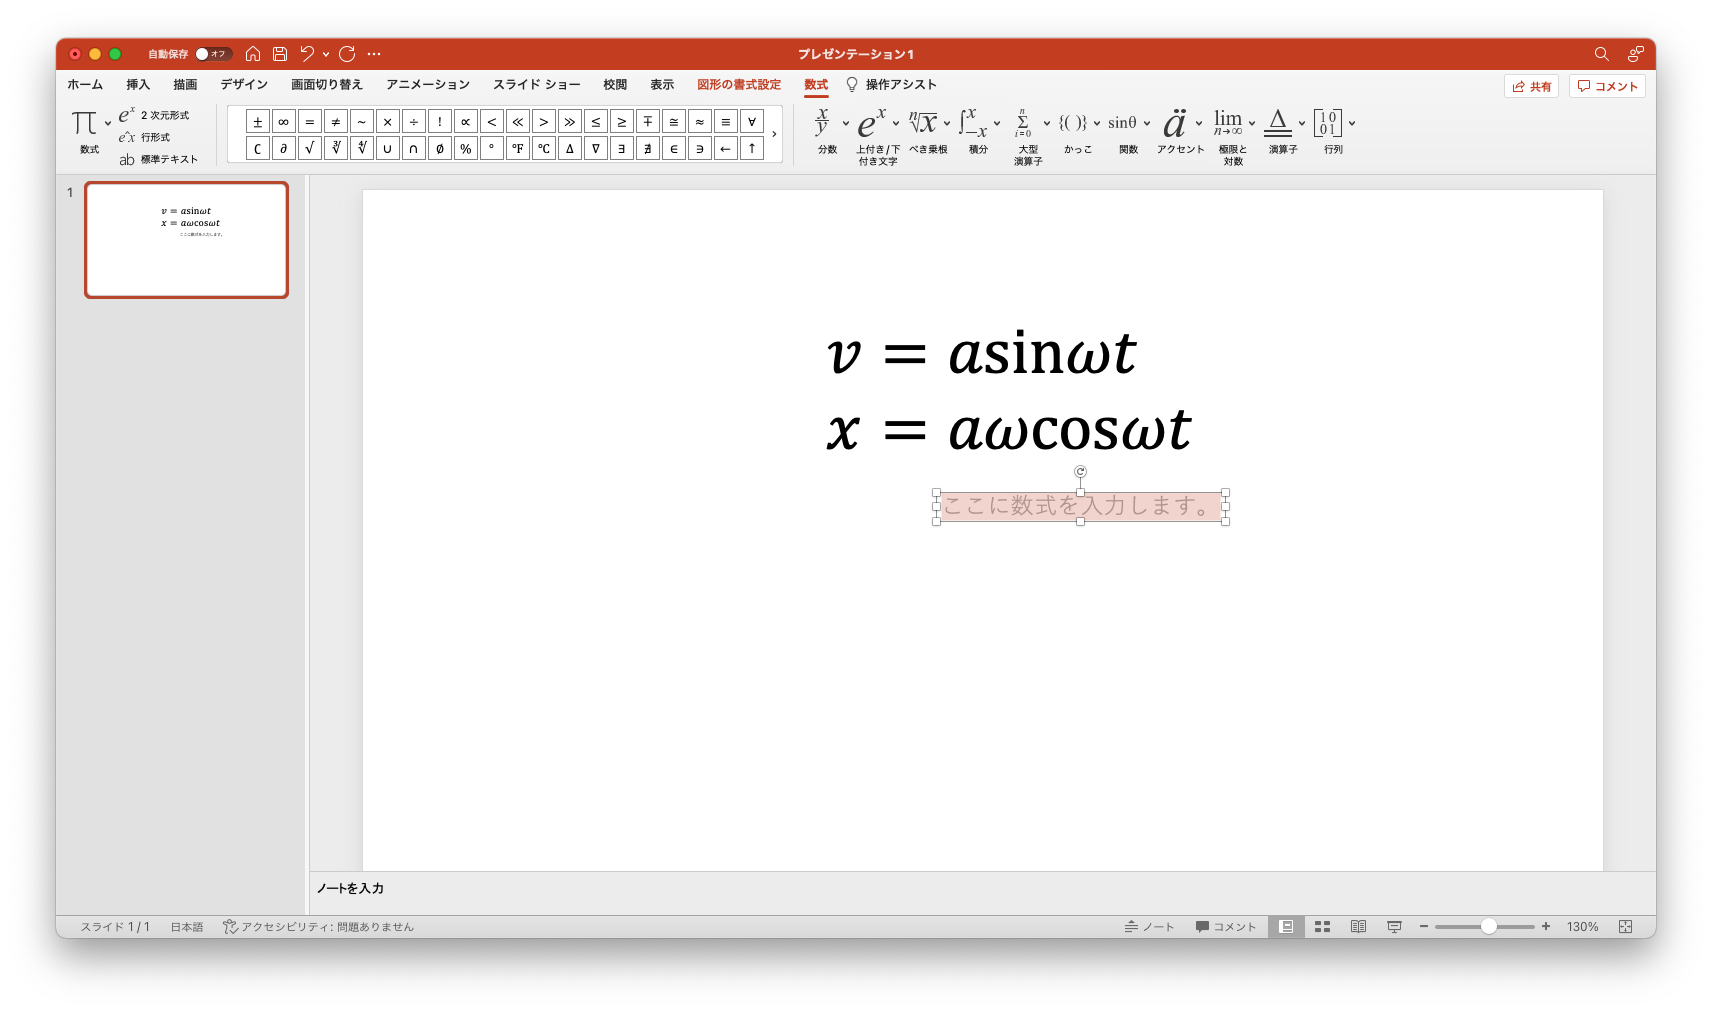
\includegraphics[scale = 0.15]{PowePoint.png}
        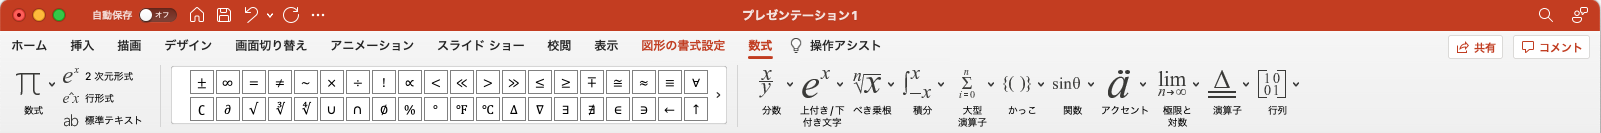
\includegraphics[scale = 0.2]{PowePoint2.png}
    \end{figure}
\end{frame}

\begin{frame}[fragile]{\LaTeX での数式の入力}
    \begin{exampleblock}{入力例}
        \begin{center}
            \verb|\[v=a\sin \omega t\]|\\
            \verb|\[x=a\omega \cos \omega t\]|
        \end{center}
    \end{exampleblock}
    \begin{exampleblock}{入力例に対する出力}
        \[v=a\sin \omega t\]
        \[x=a\omega \cos \omega t\]
    \end{exampleblock}
\end{frame}

\begin{frame}[fragile]{align環境を用いれば「綺麗」かつ「便利」}
    \begin{exampleblock}{入力例}
        \begin{verbatim}
\begin{align}
    v &= a\sin \omega t\label{式:等速円運動の速度式}\\
    x &= a\omega \cos \omega t\label{式:等速円運動の変位式}
\end{align}
式(\ref{式:等速円運動の速度式})を時間$t$で微分すると,
                    式(\ref{式:等速円運動の速度式})になる.
        \end{verbatim}
    \end{exampleblock}
    \begin{exampleblock}{入力例に対する出力}
        \begin{align}
            v & = a\sin \omega t\label{式:等速円運動の速度式}        \\
            x & = a\omega \cos \omega t\label{式:等速円運動の変位式}
        \end{align}
        式(\ref{式:等速円運動の速度式})を時間$t$で微分すると,式(\ref{式:等速円運動の変位式})になる.
    \end{exampleblock}
\end{frame}
\begin{frame}{さまざまな数式がきれいに書ける}
    \begin{exampleblock}{数式例}
        \begin{align*}
             & \lim_{a\to \infty}a_n=0\Leftrightarrow\forall \varepsilon >0\exists N\in\mathbb{N}\forall n\in\mathbb{N}(n\geq N\to (a_n-a)<\varepsilon)\tag{1学年1Q:コーシーの収束の定義} \\\\
             & \int_{a}^{b}f(x)\textrm{dx}=F(b)-F(a)\tag{1学年3Q:微積分学の基本定理}                                                                                                      \\\\
             & (\mathbb{Z}_6,+)\textrm{は,アーベル群.}N=\{\{0\},\{0,2,4\},\{0,3\},\{\mathbb{Z}_6\}\}\subseteq\mathbb{Z}_6 \tag{2学年1Q:代数学概論 群論 部分群}
        \end{align*}
    \end{exampleblock}
\end{frame}
\begin{frame}{さまざまな数式がきれいに書ける}
    \begin{exampleblock}{数式例}
        \begin{align*}
            F      & = -m\omega^2x\tag{復元力}                               \\
                   & = -Kx (K\geq 0)                                         \\
            ma     & = -Kx                                                   \\\\
            \omega & =\sqrt{\dfrac{K}{m}}                                    \\
            T      & = 2\pi\sqrt{\dfrac{m}{K}}\tag{復元力による単振動の周期}
        \end{align*}
    \end{exampleblock}
\end{frame}

\subsection{参照}
\begin{frame}
    \frametitle{目次}
    \tableofcontents[currentsection,sectionstyle=show/shaded,subsectionstyle=show/shaded]
\end{frame}

\begin{frame}[fragile]{オブジェクトに付番して参照する}
    \begin{exampleblock}{入力例}
        \begin{verbatim}
\caption{適当な図}
\label{fig:適当な図}
\includegraphics{fogefoge.png}
図\ref{fig:適当な図}は,めっちゃいいよね.
    \end{verbatim}
    \end{exampleblock}
    \begin{exampleblock}{入力例に対する出力}
        \begin{figure}[h]
            \centering
            \caption{適当な図}
            \label{fig:適当な図}
            \includegraphics[scale = 0.009]{fig1.jpeg}\\
            図\ref{fig:適当な図}は,めっちゃいいよね.
        \end{figure}
    \end{exampleblock}
    図表のキャプションや,\textcolor{red}{文書中のカウンタは任意に追加変更できる.}\verb|\renewcommand,\setcounter|
\end{frame}

\begin{frame}[fragile]{参考文献例}
    \begin{exampleblock}{入力例}
        \begin{verbatim}
溝口洸熙は没個性的な大学生である.\cite{bibitem:俺のブログ}
---
\begin{thebibliography}{99}
    \bibitem{bibitem:俺のブログ} 
                \url{https://mizomizo0515.hatenablog.com}
\end{thebibliography}
        \end{verbatim}
    \end{exampleblock}
    \begin{exampleblock}{出力例}
        溝口洸熙は没個性的な大学生である.[1]\\
        \textbf{参考文献}\\
        \verb|[1] https://mizomizo0515.hatenablog.com|
    \end{exampleblock}
    \textcolor{red}{参考文献は,原則文書の巻末につける.}
\end{frame}


\subsection{描画}
\begin{frame}
    \frametitle{目次}
    \tableofcontents[currentsection,sectionstyle=show/shaded,subsectionstyle=show/shaded]
\end{frame}

\begin{frame}{Ti\emph{k}Zで綺麗なグラフ}
    \begin{figure}[h]
        \caption{$v=v_0+at$}
        \label{fig:v-t2}
        \begin{tikzpicture}
            \def\G{{-1 * \t + 3}}
            \def\vtG{plot(\t,\G)}
            \coordinate (C) at (5,-2);
            \coordinate (O) at (0,0);
            \draw[name path = tShaft,thick,->,>=LaTeX](0,0)--(6.4,0)node[right]{$t$};%t軸
            \draw[name path = vShaft,thick,->,>=LaTeX](0,-2)--(0,4)node[above]{$v$};%v軸
            \draw[name path = vtGlaph,very thick,domain = 0:5,variable=\t]\vtG;
            \draw[name path = CD,dashed](5,0)node[above]{D}node[below right]{$t_2$}--(C)node[right]{C};
            \draw[name path = vC,dashed](C)--(0,-2)node[left]{$v$};
            \path[name intersections = {of = vShaft and vtGlaph, by={A}}];
            \path[name intersections = {of = tShaft and vtGlaph, by={B}}];
            \begin{scope}[on background layer]
                \fill[fill = gray!10](O)--(A)--(B)--cycle;
                \fill[fill = gray!50](B)--(C)--(5,0)--cycle;
            \end{scope}

            \foreach \P in {A,B} \fill[black] (\P) circle [radius = 0.06]node[above right]{\P};
            \foreach \P in {O,C} \fill[black] (\P) circle [radius = 0.06];
            \draw(B)node[below left]{$t_1$};
            \draw(A)node[left]{$v_0$};
            \draw(O)node[left]{O};
            \draw ($(O)!0.5!(B)$)node[above]{\scriptsize{速度正}};
            \draw ($(5,0)!0.5!(B)$)node[below]{\scriptsize{速度負}};
        \end{tikzpicture}
    \end{figure}
\end{frame}

\begin{frame}{Ti\emph{k}Zで綺麗なグラフ}
    \begin{figure}[h]
        \caption{$x=v_0t+\dfrac{1}{2}at^2$}
        \label{fig:v-t3}
        \begin{tikzpicture}
            \def\G{{-1/2 * (\t)^2 + 3*\t}}
            \def\vxG{plot(\t,\G)}
            \draw[name path = tShaft,thick,->,>=LaTeX](0,0)--(6.4,0)node[right]{$t$};%t軸
            \draw[name path = xShaft,thick,->,>=LaTeX](0,0)--(0,5)node[above]{$x$};%x軸
            \coordinate (O) at (0,0);
            \fill[black] (O) circle [radius = 0.06];
            \draw[name path = vxGlaph1,thick,domain = 0:3,variable=\t,samples = 100]\vxG;
            \draw[name path = vxGlaph2,very thick,red,domain = 3:6,variable=\t,samples = 100]\vxG;
            \draw[dashed](3,9/2)--(3,0)node[below]{$t_1$};
            \draw[dashed](0,9/2)node[left]{$x_1$}--(3,9/2);
            \fill[black](3,9/2) circle [radius = 0.06];
            \fill[black](6,0) circle [radius = 0.06]node[below]{$t_2$};
            \draw (0,0)edge[bend right = 20]node[below]{\scriptsize{正の向きに進む}}(3,0);
            \draw (3,0)edge[bend right = 20]node[below]{\scriptsize{負の向きに進む}}(6,0);
        \end{tikzpicture}
    \end{figure}
\end{frame}

\begin{frame}[fragile]{Ti\emph{k}Zで綺麗なグラフ}
    \begin{figure}[h]
        \centering
        \begin{tikzpicture}
            \node[rounded corners,fill=cyan!10,rectangle,minimum size=1cm](0){\verb|args[0]|};
            \node[rounded corners,fill=cyan!10,rectangle,minimum size=1cm,right=1cm of 0](1){\verb|args[1]|};
            \node[right=0.5cm of 1](d){\dots};
            \node[rounded corners,fill=cyan!10,rectangle,minimum size=1cm,right=0.5cm of d](n){\verb|args[n]|};
            \node[inner sep=0.3cm,fit={(0)(1)(d)(n)}](wrap_main){};
            \node[inner sep=0cm,above=0.3cm of wrap_main.north west](caption_main){\verb|main|};
            \node[draw,rounded corners,fit={(wrap_main)(caption_main)}](plate_main){};

            \node[diamond,fill=red!10,minimum size=1cm,below=1cm of plate_main](Search){検索};

            \draw[white,line width=4pt,bend right=15]
            (0)     edge (Search)
            (1)     edge (Search)
            (n)     edge (Search);
            \draw[->,bend right=15,dashed]
            (0)     edge (Search)
            (1)     edge (Search)
            (n)     edge (Search);

            \draw[white,line width=4pt,bend right=15]
            (Search)     edge (0)
            (Search)     edge (1)
            (Search)     edge (n);
            \draw[->,bend right=15]
            (Search)     edge (0)
            (Search)     edge (1)
            (Search)     edge (n);
        \end{tikzpicture}
    \end{figure}
\end{frame}

\subsection{利用環境}
\begin{frame}
    \frametitle{目次}
    \tableofcontents[currentsection,sectionstyle=show/shaded,subsectionstyle=show/shaded]
\end{frame}

\begin{frame}[fragile]{利用環境}
    \begin{block}{作成・編集}
        \verb|filename.tex|というファイルに,適当なエディタで文字を打つのみ.OSに依存しない作成環境.
    \end{block}
    \begin{block}{出力}
        \LaTeX の出力は,基本的にPDFなので,環境に依存しない.\\
        また,\LaTeX のコンパイル環境はWindows,macOS,Linuxにインストール可能.
    \end{block}
\end{frame}

\section{個人的}
\subsection{感想}
\begin{frame}
    \frametitle{目次}
    \tableofcontents[currentsection,sectionstyle=show/shaded,subsectionstyle=show/shaded]
\end{frame}

\begin{frame}{個人的感想}
    \begin{block}{レジュメ用途が最適}
        文字数や情報量が多い資料は,伝えたい重要なことが目立ちにくい.そのため,Beamerを利用した資料は,レジュメとして手元に配布する用途として作成することが最適であると考える.\\
    \end{block}
\end{frame}
\subsection{提案}
\begin{frame}
    \frametitle{目次}
    \tableofcontents[currentsection,sectionstyle=show/shaded,subsectionstyle=show/shaded]
\end{frame}
\begin{frame}[fragile]{Keynote}
    プレゼンテーションアプリで一番おすすめは"Keynote"(Apple).\TeX コマンドで数式を入力できる.
    \ovalbox{Command+Option+E}で数式作成Boxを作成.
    \begin{figure}[h]
        \centering
        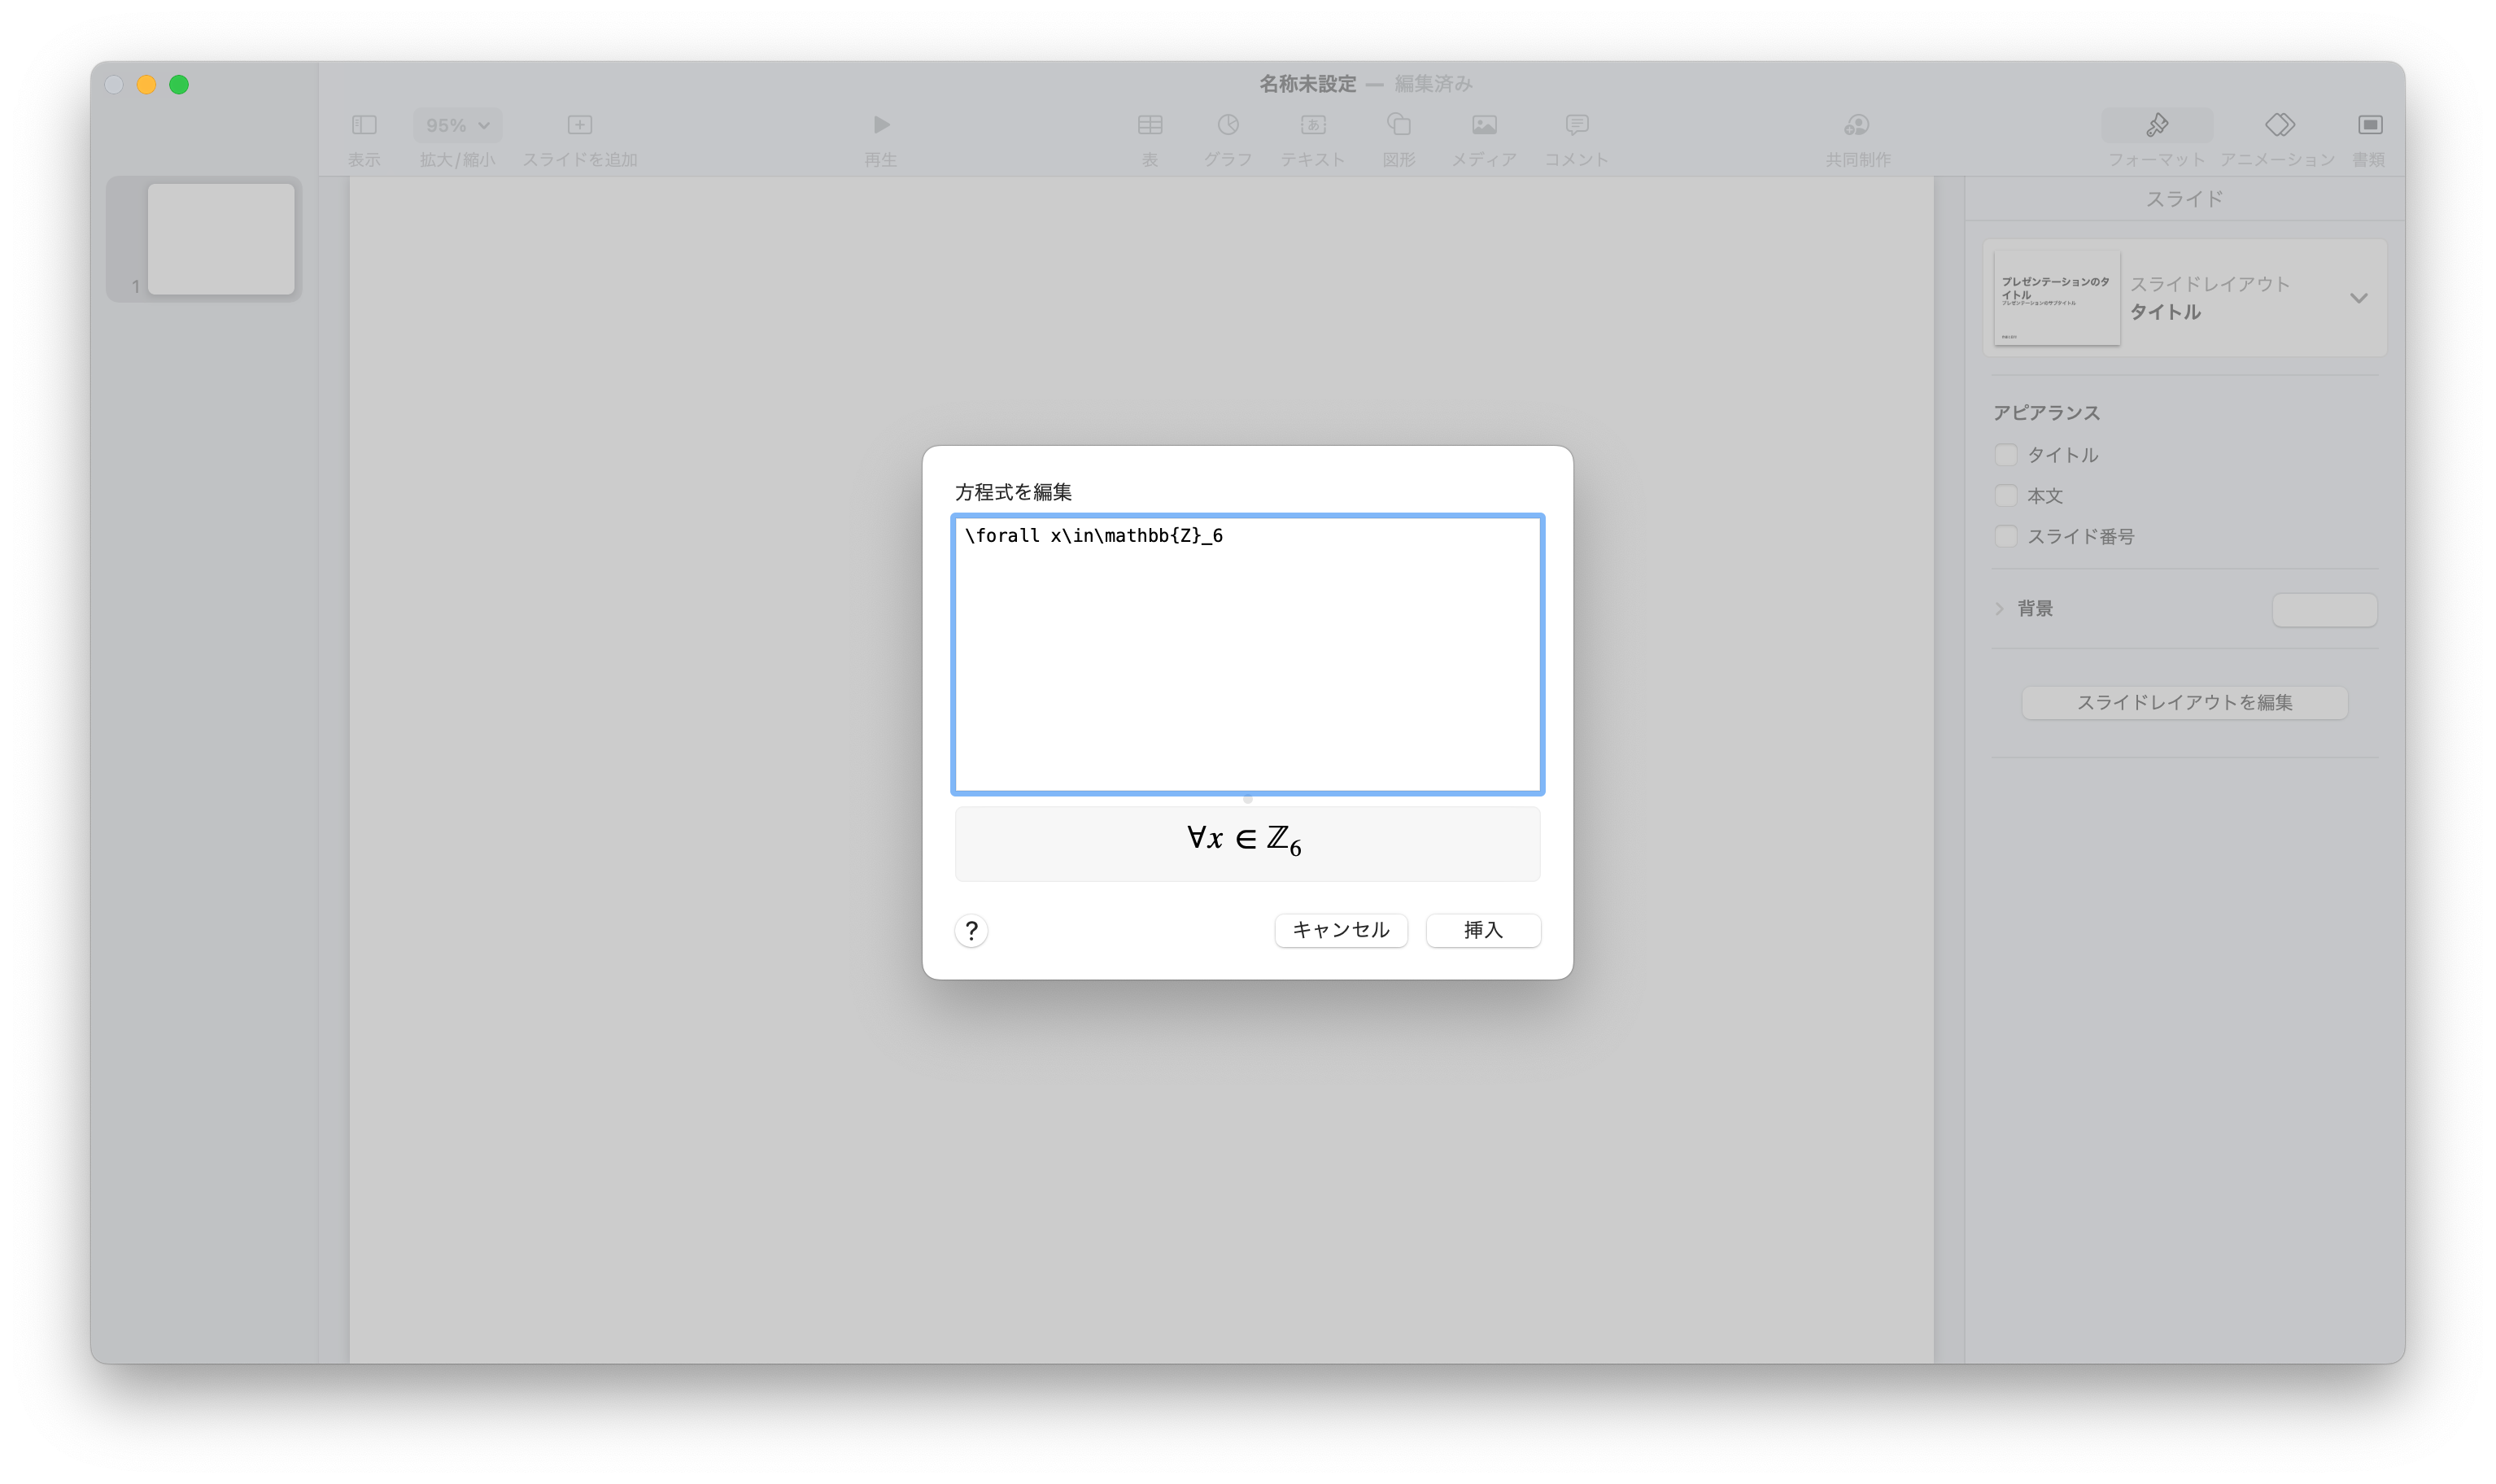
\includegraphics[scale = 0.2]{fig2.png}
    \end{figure}
\end{frame}


\section{参考文献}
\begin{frame}{参考文献}
    \begin{thebibliography}{99}
        \bibitem{label3} \url{https://ja.wikipedia.org/wiki/LaTeX}\\
        \hspace{3em}Wikipedia(非推奨) \today 最終確認
        \bibitem{label1} \url{https://ayapin-film.sakura.ne.jp/LaTeX/Slides/Beamer-tutorial.pdf}\\
        \hspace{3em}Beamer 読本 東京電機大学 \today 最終確認
        \bibitem{label2} \url{https://texwiki.texjp.org/}\\
        \hspace{3em}\TeX Wiki \today 最終確認
    \end{thebibliography}
\end{frame}
\end{document}
